\addsec{Auswertung der Schülerumfrage}
\normalsize
Im Zeitraum vom 17. 11. 2020 bis 26. 11. 2020 führte unsere Seminarfachgruppe eine anonyme Online-Umfrage für Schüler des hennebergischen Gymnasiums "Georg Ernst" durch. Jegliche erhobenen Daten wurden ausschließlich im Rahmen dieser Arbeit benutzt und nach der entsprechenden Auswertung gelöscht. Zum Zeitpunkt der Auswertung haben insgesamt 147 Schüler teilgenommen.\\\\
Wenn mehrere Antworten angegeben wurden, zählt jede je nach Frage entweder als eine Stimme(*) oder eine Stimme wird anteilmäßig auf die genannten Antwortmöglickeiten verteilt(**).\\\\\\\\\\\\\\\\



Würden Sie die folgenden Produkte eher Online oder vor Ort kaufen? (1)\\\\
\begin{figure}[H]
    \begin{center}
        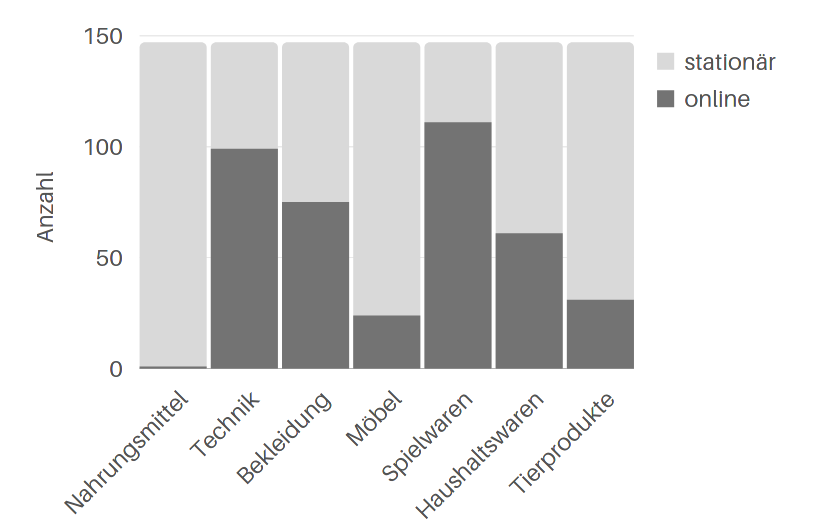
\includegraphics[width=12.5cm]{media/schuelerumfrage/1.png}
    \end{center}
\end{figure} 



\newpage\noindent Haben Sie schon einmal etwas Online bestellt, wenn ja über welche Plattform? (2)\\
\begin{figure}[H]
    \begin{center}
        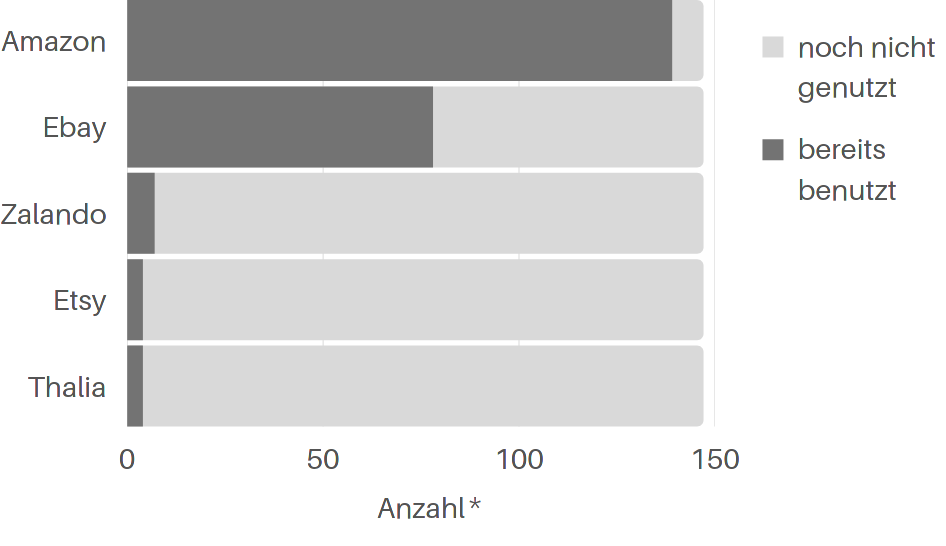
\includegraphics[width=11.5cm]{media/schuelerumfrage/2.png} 
    \end{center}
\end{figure}

\noindent weitere genannte Plattformen:
\begin{itemize}
 \item Zaful (3)
 \item H\&M (2)
 \item EMP (2)
 \item Intersport (2)
 \item Bershka (1)
 \item Shein (1)
 \item Maciag Offroad (1)
 \item Reifendirekt (1)
 \item Böttcher AG (1)
 \item Globetrotter (1)
\end{itemize}



\iffalse \newpage\noindent Gibt es Artikel, die Sie nicht Online bestellen würden?** (3)\\\\\\
\begin{figure}[H]
    \begin{center}
        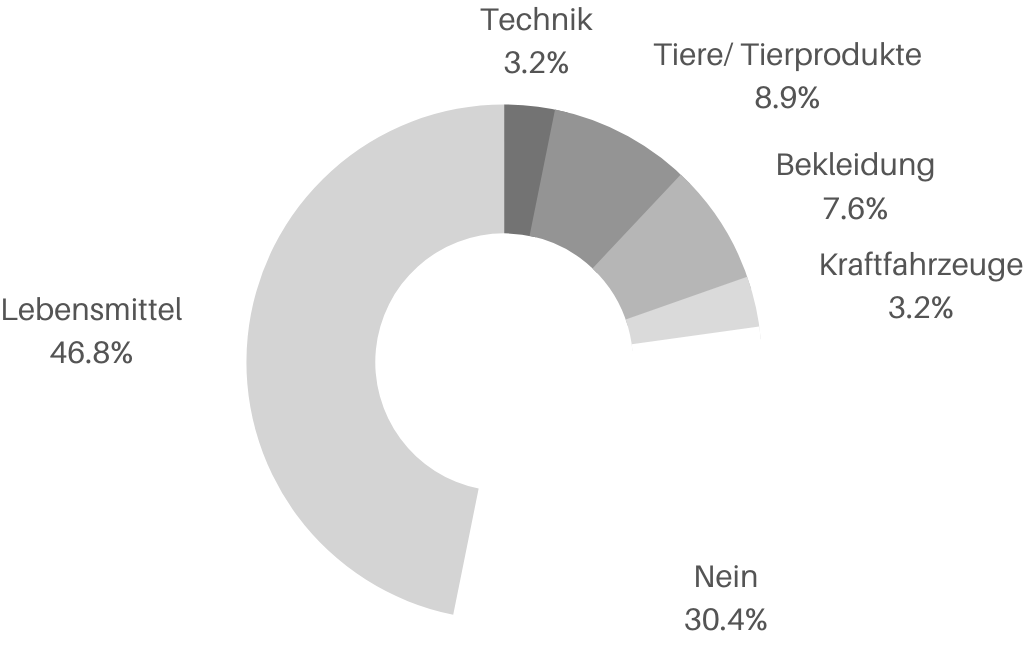
\includegraphics[width=11.5cm]{media/schuelerumfrage/3.png}
    \end{center}
\end{figure}
\vfill
\noindent weitere genannte Produkte:
\begin{itemize}
 \item Gebrauchtwaren (3)
 \item Mietwohnung (1)
\end{itemize}
\vfill\vfill\vfill\vfill \fi



\iffalse \newpage\noindent Wie beschreiben Sie ihre Erfahrungen mit dem Onlinehandel? (4)\\\\\\
\begin{figure}[H]
    \begin{center}
        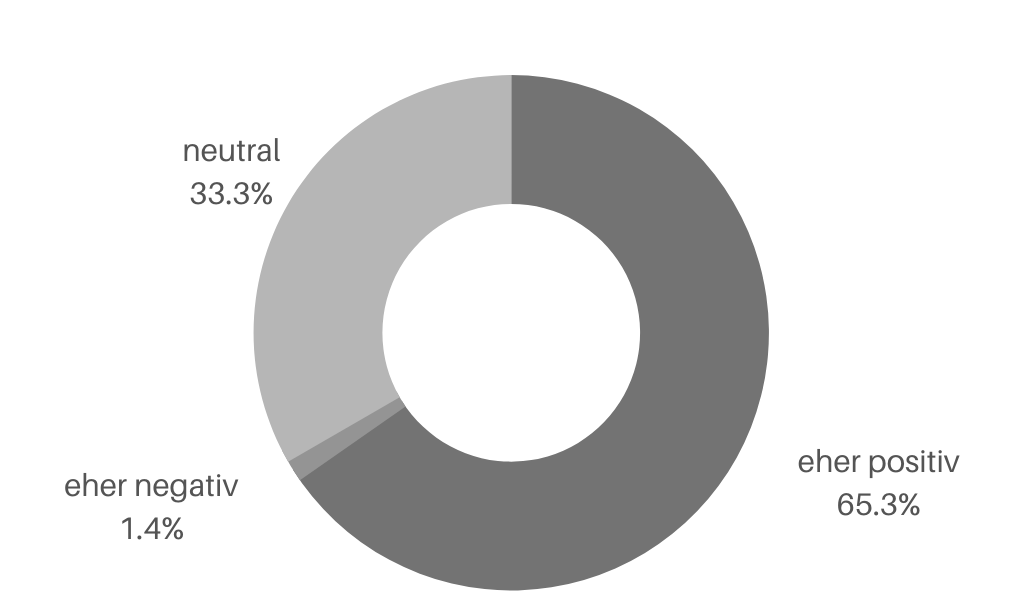
\includegraphics[width=11.5cm]{media/schuelerumfrage/4.png}
    \end{center}
\end{figure} \fi



\iffalse \newpage\noindent Ist das Kaufangebot im schleusinger Umkreis ausreichend? Falls nein, was fehlt?** (5)\\
\begin{figure}[H]
    \begin{center}
        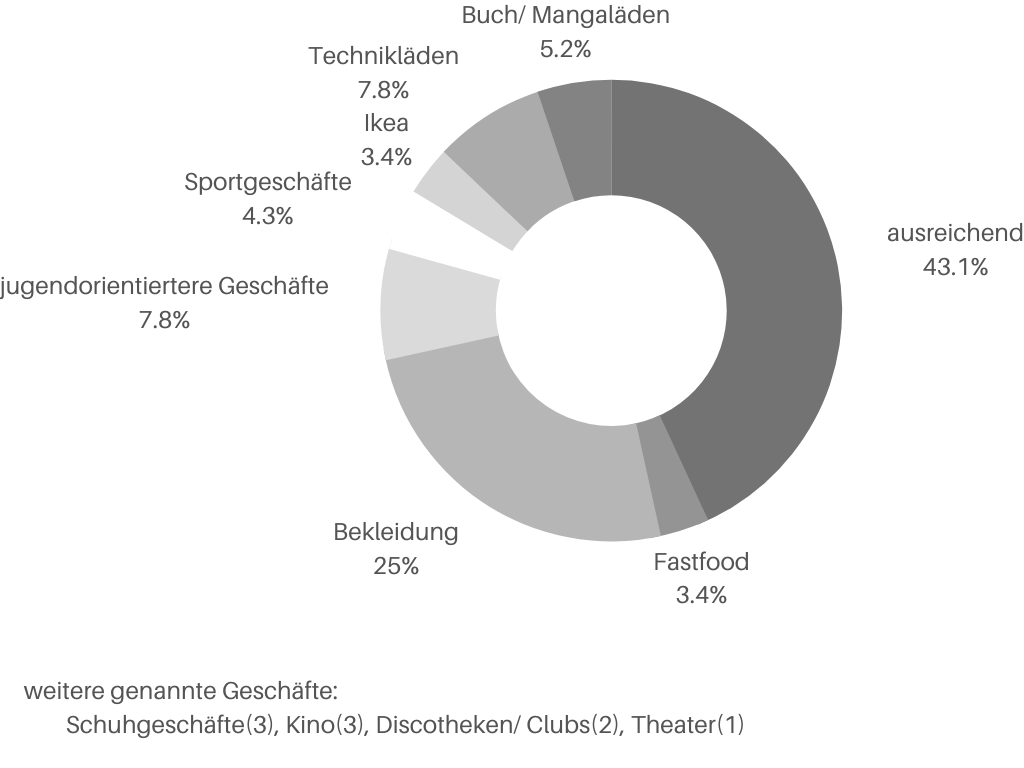
\includegraphics[width=15cm]{media/schuelerumfrage/5.png}
    \end{center}
\end{figure} \fi



\newpage\noindent Weichen Sie und ihre Familie beim Einkaufen aufgrund des Angebots auf andere Städte in der Umgebung aus? (6)\\
\vfill
\begin{figure}[H]
    \begin{center}
        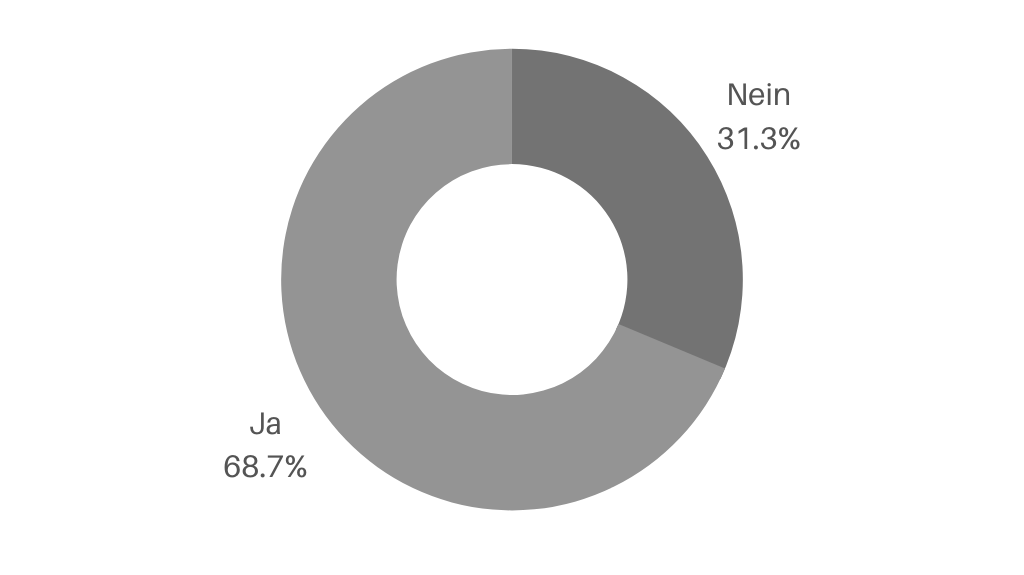
\includegraphics[width=12cm]{media/schuelerumfrage/6.1.png}
    \end{center}
\end{figure}
\vfill
\begin{figure}[H]
    \begin{center}
        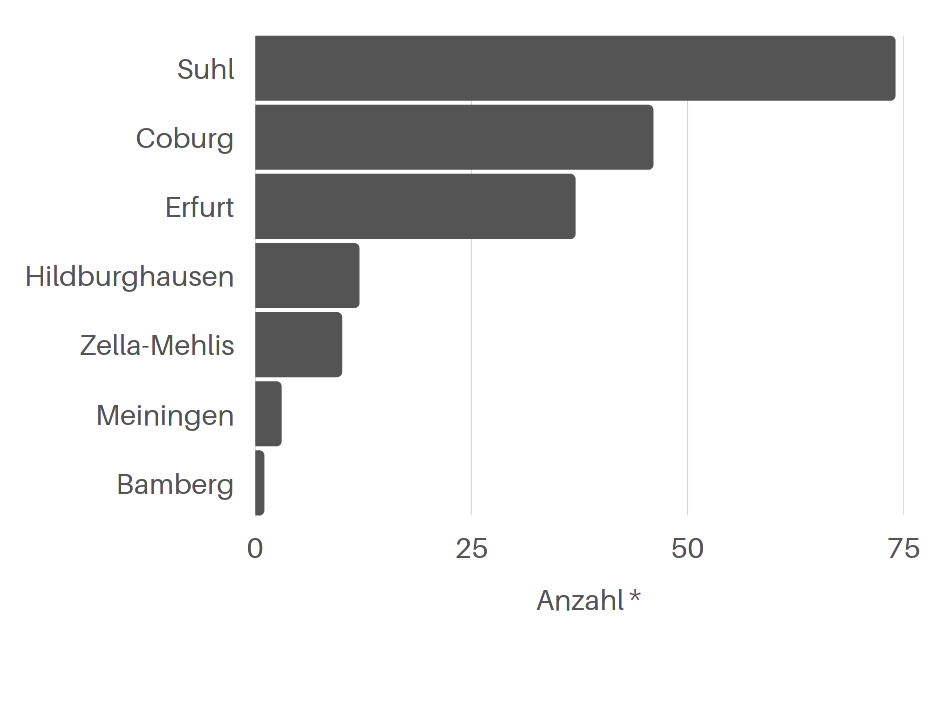
\includegraphics[width=12cm]{media/schuelerumfrage/6.2.png}
    \end{center}
\end{figure}
\vfill



\newpage\noindent Welche Produkte/ Änderungen im Verkaufsprozess wünschen Sie sich für den Onlinehandel? (7)\\\\

\begin{figure}[H]
    \begin{center}
        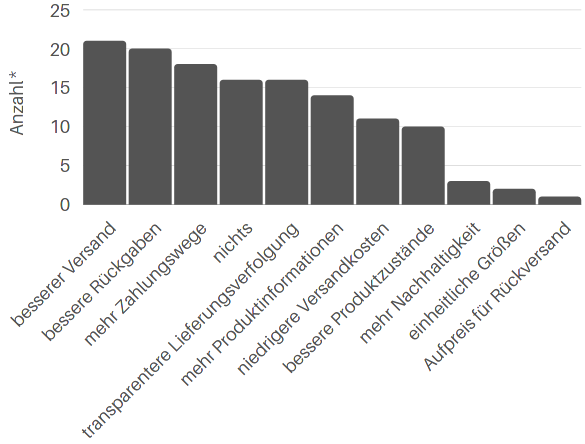
\includegraphics[width=12cm]{media/schuelerumfrage/7.png} 
    \end{center}
\end{figure}
\vfill\vfill
\noindent Auffälligkeiten:
\begin{itemize}
 \item Paypal ist als Zahlungsweg am meisten gefragt
 \item Aufpreis für Rückversand, um Umweltbelastung zu verringern
 \item oft online-spezifisches und geringe Schnittmenge mit Frage 8
 \end{itemize}
\vfill\vfill\vfill\vfill



\newpage\noindent Welche Produkte/ Änderungen im Verkaufsprozess wünschen Sie sich für den lokalen Handel? (8)\\
\vfill
\begin{figure}[H]
    \begin{center}
        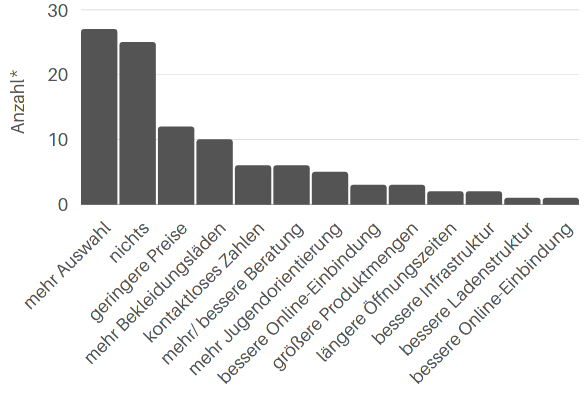
\includegraphics[width=12cm]{media/schuelerumfrage/8.png}
    \end{center} 
\end{figure}
\vfill\vfill
\noindent Auffälligkeiten:
\begin{itemize}
 \item sehr oft "keine Ahnung"
 \item ausschließlich eine größere Auswahl wird oft genannt
 \item wenig bis keine Überschneidung mit Antworten aus Frage 7
 \end{itemize}
\vfill\vfill\vfill\vfill



\iffalse \newpage\noindent Welche Stärken sehen Sie bzgl. des stationären Einzelhandels im ländlichen Bereich? (9)\\
\begin{figure}[H]
    \begin{center}
        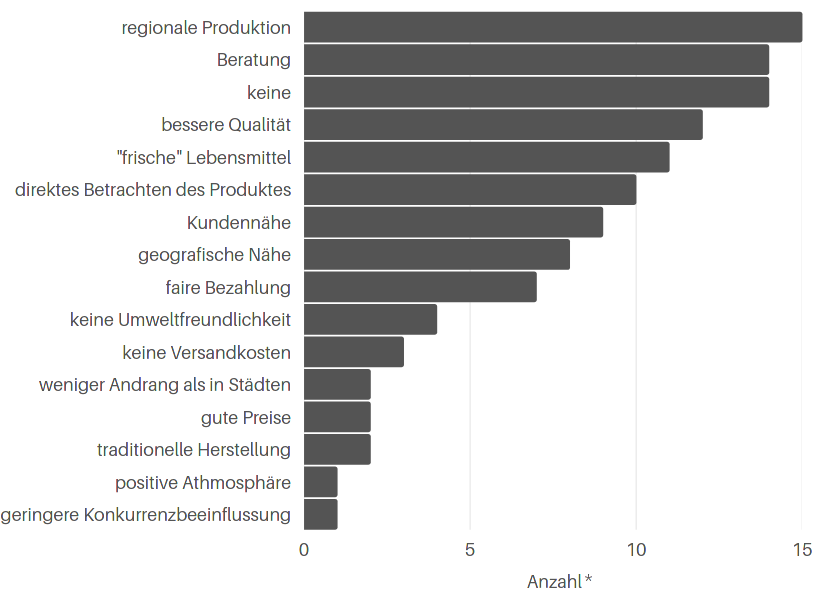
\includegraphics[width=15cm]{media/schuelerumfrage/9.png}
    \end{center}
\end{figure} \fi



\iffalse \newpage\noindent Kaufen Sie und ihre Familie Gebrauchsgegenstände (mehrfach verwendbare, z. B. Autos, Fernseher usw.) größtenteils neu oder gebraucht? (10)\\

\begin{figure}[H]
    \begin{center}
        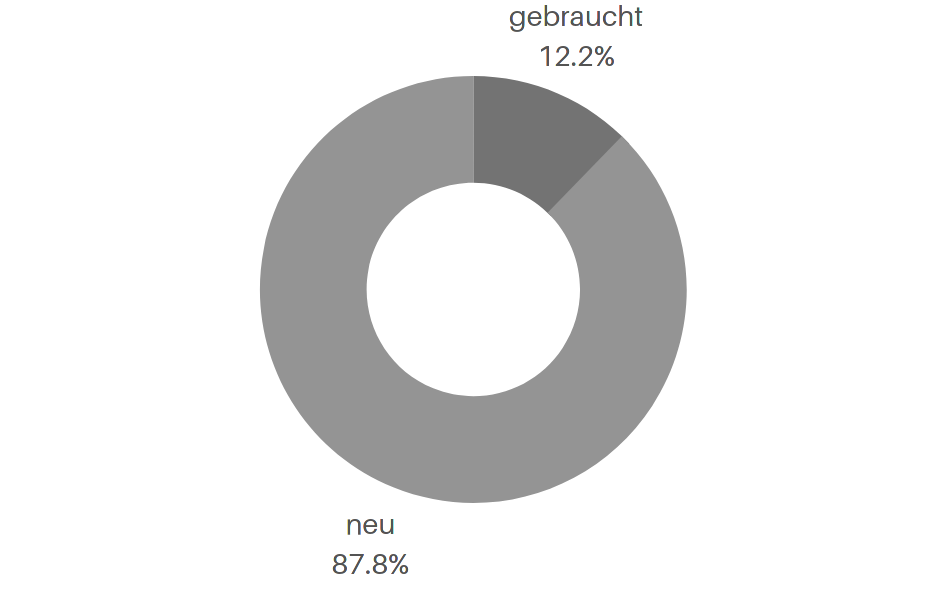
\includegraphics[width=12cm]{media/schuelerumfrage/10.png}
    \end{center}
\end{figure} \fi



\iffalse \newpage\noindent Was ist für Sie relevanter? Der Onlinehandel oder der stationäre Einzelhandel? (11)\\

\begin{figure}[H]
    \begin{center}
        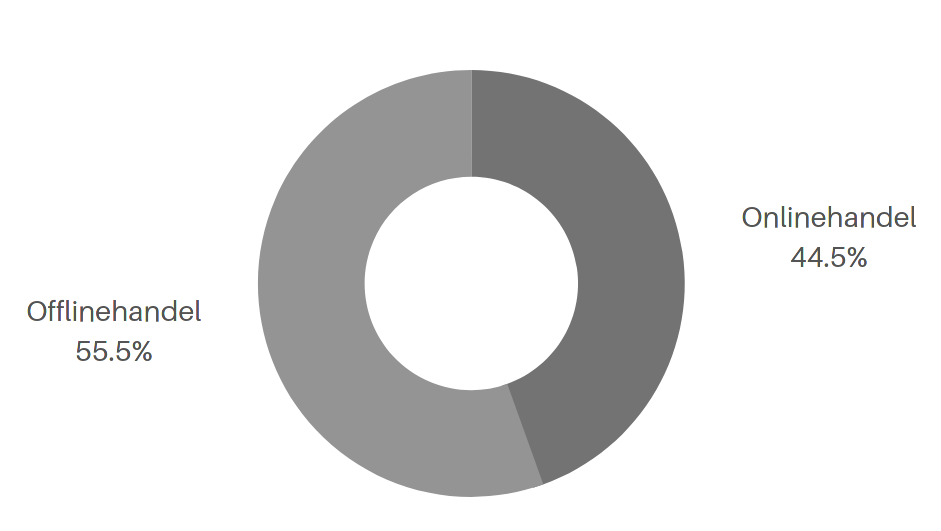
\includegraphics[width=12cm]{media/schuelerumfrage/11.png}
    \end{center}
\end{figure} \fi



\iffalse \newpage\noindent Welche Probleme/ Komplikationen sehen sie beim Kauf von Artikeln Online? (12)
\begin{figure}[H]
    \begin{center}
        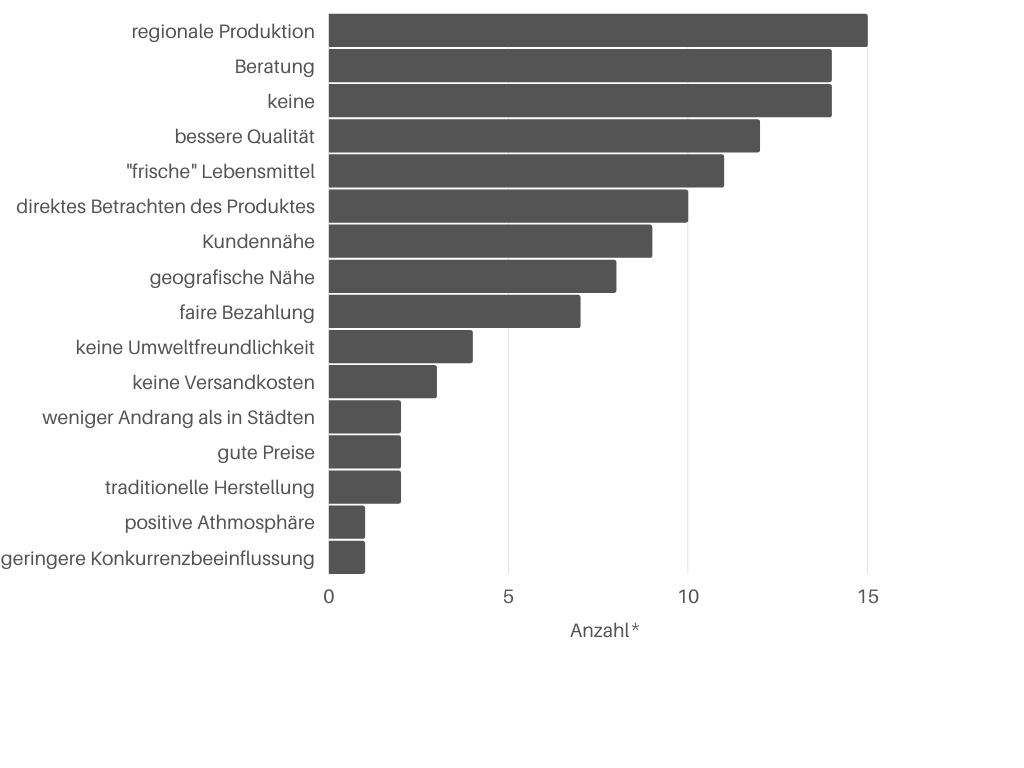
\includegraphics[width=17cm]{media/schuelerumfrage/12.png}
    \end{center}
\end{figure} \fi



\iffalse \newpage\noindent Wie schätzen sie ihre Preissensibilität ein? (13)\\
 
\begin{figure}[H]
    \begin{center}
        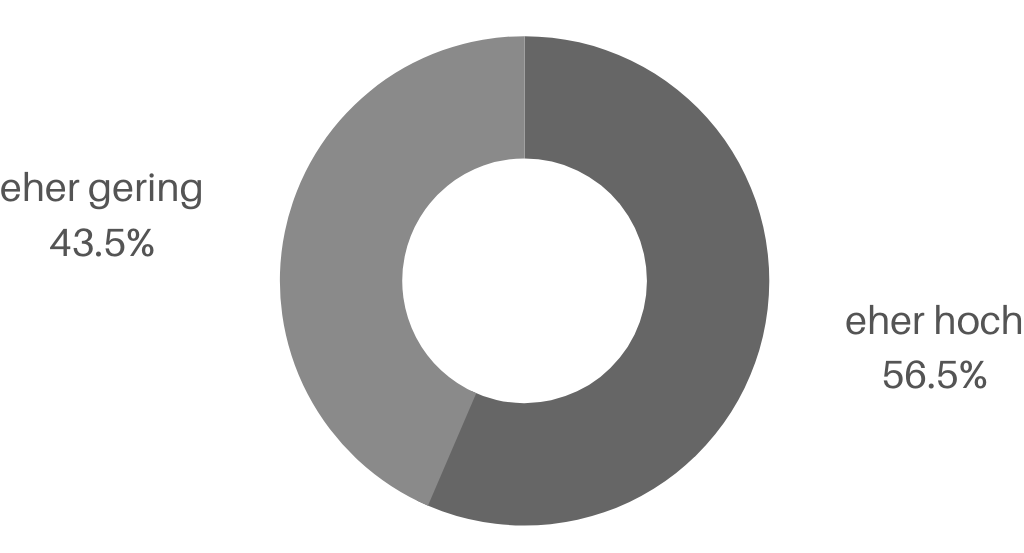
\includegraphics[width=9cm]{media/schuelerumfrage/13.png}
    \end{center}
\end{figure} \fi 



\newpage\noindent Haben sich ihre Kaufgewohnheiten während der Corona-Zeit geändert? (14)\\\\\\

\begin{figure}[H]
    \begin{center}
        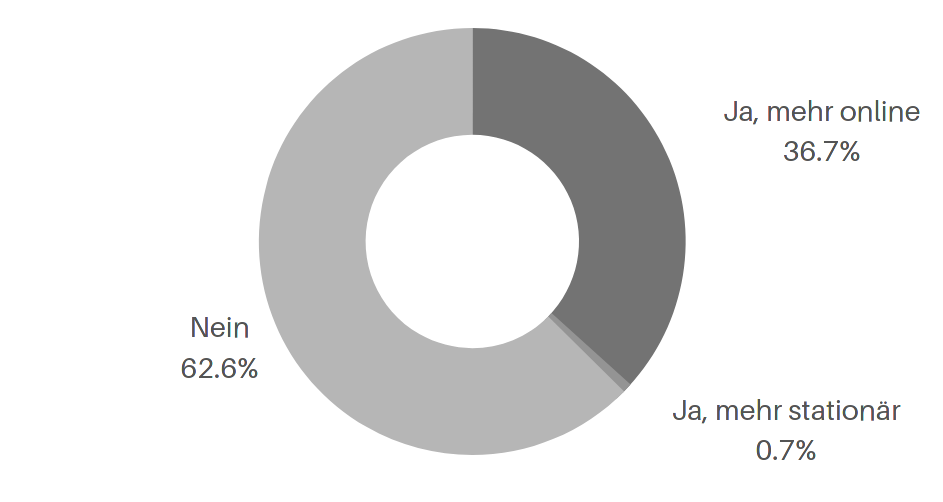
\includegraphics[width=12cm]{media/schuelerumfrage/14.png}
    \end{center}
\end{figure}

\iffalse \noindent Wann haben Sie das erste mal etwas online gekauft? (15)\vfill

\begin{figure}[H]
    \begin{center}
        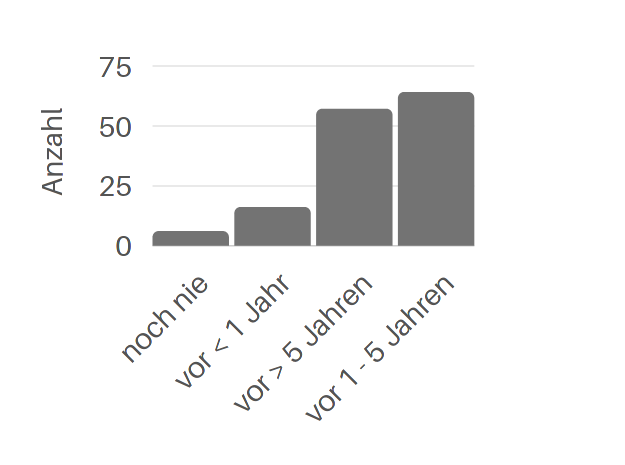
\includegraphics[width=8cm]{media/schuelerumfrage/15.png}
    \end{center}
\end{figure} 
\vfill \fi
\newpage









